\section{A Solution for Access Control in Big Data Scenarios}\label{sec:access}

Our methodology is based on two key pillars: on one side, we define an \textit{attribute-based access control model} that offers flexible fine grained authorization capabilities and exploits XACML notion of obligation to introduce preemptive data transformations that in a collaborative big data scenario are more suitable that denying data access.  On the other side,  differently from our previous work \cite{medes2021} where access control was done only at ingestion time, we monitor every data processing operation along the whole pipeline (see requirement {\bf R3}).

\subsection{Access Control Policy Model}\label{sec:ACmodel}

Recently, attribute-based access control has gained a lot of attention thanks to its highly customized ability to express dynamic and fine grained rules. Instead of assigning capabilities (i.e., action/object pairs) directly to a subject or to its role, policies rules specify under which conditions access is granted or denied. Rules are specified in terms of attributes of the subject, attributes of the object and environment conditions, with the advantage of allowing policies to be created and managed without direct reference to potentially numerous subjects and objects, and subject and objects to be provisioned without reference to a policy (requirement {\bf R6}). This approach also minimizes the number of policy rules needed (requirement {\bf R11}). Finally, by playing with attributes and environment conditions, we are able to express policies satisfying the requirements listed in Section \ref{sec:accesscontrol_req} and the peculiarities of big data scenarios. 

Our access control model then extends the policy structure of traditional attributed-based access control systems with two features:
\begin{itemize}
\item XACML optional obligations \cite{XACML3.0} specifying actions that must be performed before the policy is enforced and not directly associated with the controlled data become mandatory and are used to express data transformations that sanitize data resources to guarantee a minimum level of access to data. 
\item the evaluation of a policy rule always ends with an allow answer. Indeed, data protection is guaranteed by means of data transformations. 
\end{itemize}

As in any attribute-based access control model, the key elements of our model are defined as follows:
\begin{itemize}
\item XACML optional obligations \cite{XACML3.0} specifying actions that must be performed before the policy is enforced and not directly associated with the controlled data become mandatory and are used to express data transformations that sanitize data resources to guarantee a minimum level of access to data (requirement {\bf R8}). 
\item the evaluation of a policy rule always ends with an allow answer. Indeed, data protection is guaranteed by means of data transformations (requirement {\bf R10}). Obviously, deny access to data can happen in extreme cases when data transformations delete all data resources\footnote{In case of a data transformation function returning an empty dataset, the pipeline is not broken.}. 
\end{itemize}

As in any attribute-based access control model, the key elements of our model are defined as follows:
\begin{itemize}
\item A {\it subject} is a user or the service provider of a job that issues access requests to perform operations on objects. Subjects may have one or more attributes of the form (\textit{aname}, \textit{avalue}) pair, with \textit{aname} the name of the attribute and \textit{avalue} its value. In our case, there is always at least one attribute, specifying the organisation the subject belongs to. We use the notation \textit{u.aname} to refer to the value of attribute named \textit{aname}. For short, we use the notation $u@X$ to specify user $u$ belonging to organization $X$, i.e., to express the value of  \textit{u.organization}. 
\CH{credo abbia senso specificare dei subject predefiniti tipo any, none e admin, anche dei service provider predefiniti come kafka, hbase, hive. Lo faccio qui o nell'esempio?}

\item An {\it object} is any data whose access is governed by the policy (requirement {\bf R4}). It can be a file (e.g., a video, text file, image, etc.), a database, a table, a column, a raw, or a cell of a table. Like subjects, objects are assigned one or more attributes and have at least one, specifying the organization the object belongs to, expressed with the same notation $o@X$ for object $o$ belonging to organization $X$.

\item An {\it action} is any job that can be performed within a big data framework, ranging from classical atomic operations on a database (e.g, CRUD operations varying depending on the data model) to coarser operations such as an Apache Spark DAG, an Hadoop MapReduce, an analytics function call, or a pipe offered by a different service provider. 

\item The {\it environment} is defined by a set of dynamic attributes related to the specific context, such as time of the day, location, ip address, risk level, etc. \CH{mettere degli attributi piu' sensati, come normal e critical situation}. 

\end{itemize}

The access control policy is then defined as a set of policy rules expressing access conditions based on the key elements and their attributes. As mentioned earlier, the novelty of our model is in the exploitation of suitable data transformation functions that are applied to the target resource in order to sanitize it before access is given (requirement {\bf R8}).
As a consequence, when a subject makes an access request to a resource (i.e., an object), the policy rule matching the access request is evaluated, and the access is given after one or more data transformations are performed (requirement {\bf R10}). Obviously, deny access to data can happen in extreme cases when data transformations delete all data resources\footnote{In case of a data transformation function returning an empty dataset, the pipeline is not broken.}. 



\begin{definition}[Policy Rule]
A {\it policy rule} is a predicate {\it policy\_rule$_{obj}$(subj, action, env, datatrans)} defined as:
\begin{verbatim}
if (cond_expr == true)
then datatrans
\end{verbatim}
where {\tt cond\_expr} is a propositional boolean expression built on composition of mathematical operators ($>,<, =, +, -, *, /$), logical operators ($\land,\lor,\neg$), set operators ($\in,\subset,\subseteq,\supset, \supseteq \cup,\cap$) and logical quantifiers ($\forall, \exists$) on the resource \textit{obj} and on arguments \textit{subj}, \textit{action} and \textit{env} and their attributes. \texttt{datatrans} are functions transforming da\-ta resources in different ways, mainly to protect against information leakage. \CH{da sistemare rendendo piu' leggibile, da decidere se va bene che i permessi siano dati come ACL}
\end{definition}

Transformation functions range from pruning and reshaping to encrypting/decrypting or anonymizing the full resource or part of it. Thus, data protection is obtained by removing or obfuscating sensitive attributes rather than denying access to full data. In section \ref{sec:dataTransformations}, we define a taxonomy of data transformations based on the security property that has to be guaranteed.
The transformation function can be applied to the full resource or to part of it, either a single attribute or a set of attributes. For example, in case of structured data it can be applied to a single cell, to (one or more) rows or columns, either to the entire table. The target of the transformation function is given as parameter to the function.

In attribute-based access control model, policies are limited only by the computational language and the richness of the available attributes. In our case, we exploit the {\it environment} field of our model to contain the dynamic information on actual coalitions to express coalitions.

\begin{definition}[Coalition]
A coalition $C$ is a set of organizations $o\in O$, with $O$ the set of the organizations associated to the specific scenario.
\end{definition}
The {\it environment} field of our model then contains both $O$ and the actual coalitions. Given an organization $o$ o, function $\textit{Coalition}(O)$ returns the set of coalitions an organization $o\in O$ is part of, i.e, $\textit{Coalition}(o)=\{ C | o \in C\}$. In a coalition resource sharing is achieved by the distribution of access permissions to coalition members. In order to simplify and speed up policy writing, it is common to define a default set of permissions rules to be applied to all coalition members. This set of rules are part of a coalition agreement.

\begin{definition}[Coalition Agreement]
A \textit{coalition a\-greement} $\textit{CA}_C$ is a set of policy rules associated to a coalition $C$ that are added to the security policy of each organization.
\end{definition}
Obviously, the rules of a coalition agreement depend on the specific nature of a coalition. For example, given a coalition $C$ between organisations that do not handle sensitive data, a default rule in the coalition agreement could be:
\vspace{0.3cm}

\noindent $\textit{policy\_rule}_{obj}(\textit{subj},\texttt{any},\textit{env},\texttt{-}) \equiv \textit{obj.organization} \in C  
 \land \textit{subj.organization} \in C 
$
\vspace{0.3cm}

\noindent expressing the fact that subjects belonging to the same coalition can have access to all data (\texttt{-} means that no transformation functions are performed before access is given).
\hl{L'esempio sotto dovrebbe parare di coalizione e coalition agreement no?}
\begin{example}
Let us consider an healthcare scenario, with an hospital $A$ storing patients' information such as patient personal information (e.g., social security number, home address, healthcare insurance, etc.), medical journals and medication records. We suppose there are three different roles among the hospital staff: doctor, nurse and administrative staff. 
They all need to access patient's data in their daily activities, but it would make sense to have specific access rules based on the role, such as:
\begin{itemize}
\item a doctor can have access only to medical journals and medication records;
\item a nurse should only have read access on medication records;
\item an administrative must have access only to patient's personal information.
\end{itemize}
In our model, we can specify the three roles as subject's attribute \textit{role}
which can have only one of three values \texttt{doctor}, \texttt{nurse}, and \texttt{admin}. Then, we can express the three policy rules as:

\vspace{0.3cm}

\noindent $\textit{policy\_rule}_{PatientData}(\textit{s},\texttt{any},\textit{env},\texttt{-}) \equiv \textit{s.role} = \texttt{doctor}
$
\vspace{0.3cm}

\noindent $\textit{policy\_rule}_{PatientData}(\textit{s},\texttt{READ},\textit{env},\texttt{medication only}) \equiv \textit{s.role} = \texttt{nurse}
$
\end{example}

\subsection{Data Annotation}

In cloud scenarios, it is common to apply metadata tags to resources to perform more sophisticated filtering or reporting on resources. A tag is a label consisting of a key and an optional value that is assigned to a resource. In our case, we exploit tagging to specify attributes of subjects, resources or contextual information. Using data annotation to enforce data protection policies has three major advantages: \begin{enumerate}
\item Metadata tagging permits to extract value also out of possibly unstructured ingested raw data. For example, it is possible to capture document semantics through tags. Thus, tagging helps in defining policies at different levels of granularity, also in case of unstructured data.
\item Tagging enables to categorize resources in different ways (e.g, by purpose, owner, environment, or other criteria), encompassing conventional database schema information. Even relationships between attributes of different data sets can be indicated as tags, without the need of, computationally expensive, data normalization. 
\item Tags can also be used to express access control related attributes, such as data sensitivity or multi-level security policies by means of owner-defined security levels, or role-based policies. 
\end{enumerate}

When using tagging for access control in a distributed scenario, it is important to devise a consistent set of tag keys, that is, a common vocabulary. However, which tags to apply to which resources differs depending on the specific use case, working environment, or context.  Table~\ref{tab:tags} provides an example of a common vocabulary at the basis of tag-based access control policies. For instance, use case {\em privacy classification} should be used every time data privacy must be protected, that is, every time personal data are involved. Data privacy generally refers to the ability of a person to determine when, how, and to what extent her personal information can be shared with or communicated to others. According to the General Data Protection Regulation (GDPR) \cite{EUdataregulations2018}, personal data are any information relating to an identified or identifiable natural person (called data subject). Based on this definition and on the technological advances that have improved data collection and analytics, personal data (Personally Identifiable Information - PII) fall into three categories: {\em i)} explicit identifiers, any information that directly identifies individuals with certainty, such as national ID, assurance number, phone number, passport number; {\em ii)} quasi identifiers, a set of data attributes that could jointly or uniquely identify a subject when combined with publicly available data, such as ZIP code, date of birth, and address; {\em iii)} sensitive information, data related to a person without directly identifying her but that, if linked to an individual, reveals sensitive aspects of her private life (e.g., religion belief, health information, legal issues).







\subsection{Data Transformation}\label{sec:dataTransformations}




\subsection{Access Control Enforcement}
Figure~\ref{fig:smet} shows how the access control model presented in section \ref{sec:ACmodel} is integrated in the big data processing system of Figure~\ref{fig:BDpipeline}. 

\begin{figure}[!t]
	\centering
	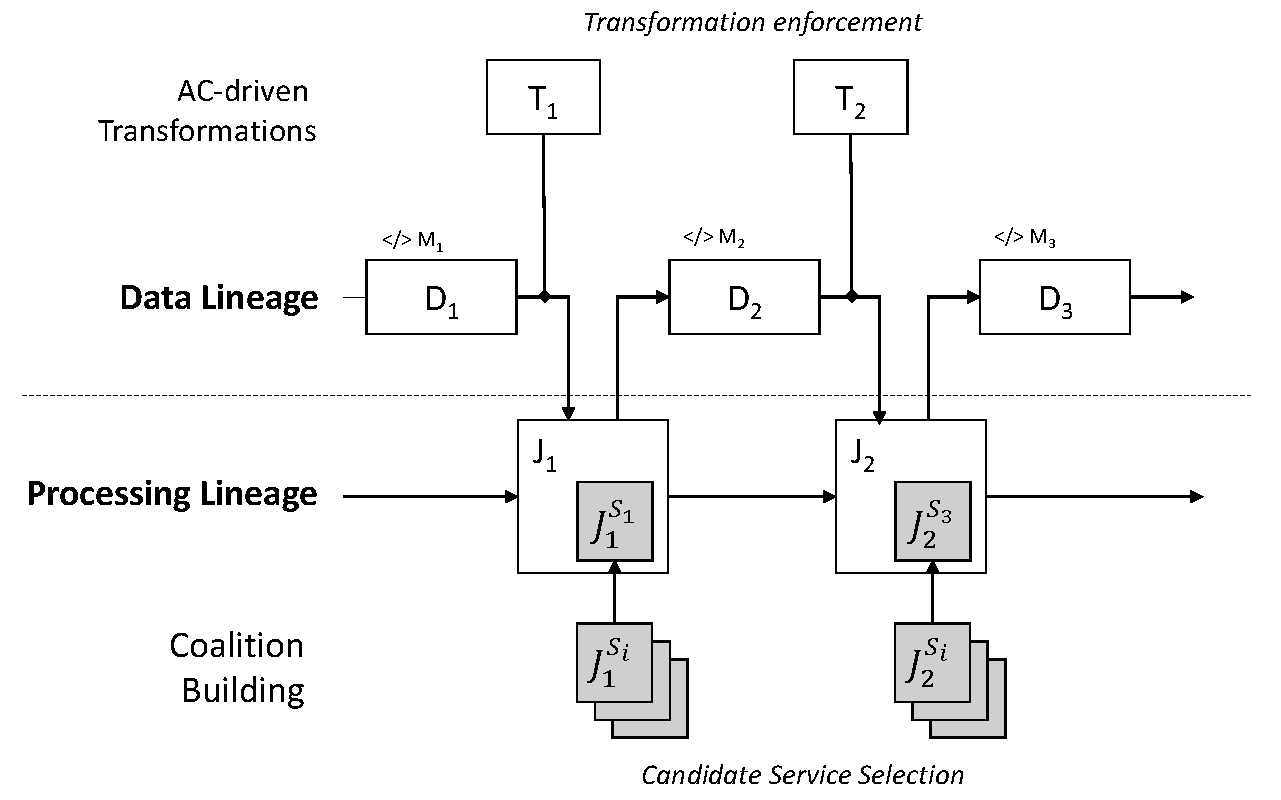
\includegraphics[width=0.48\textwidth]{meth.pdf}
\caption{Access Control Enforcement process.}
	\label{fig:smet}
\end{figure} 


Data lineage is a set of complex relationships between datasets $D_i$ and jobs $J_i$ in a pipeline.  The picture shows how policy enforcement works along the data lineage obtaining data protection by means of AC and transformations prior to feed data to a processing job.
Along the pipeline, with data flowing from data sources to computation, access control enforcement works as follows:
\begin{enumerate}
\item When $D_i$ has to be processed by job $J_i$ provided by a service provider $S_j$, an access decision has to be taken.
\item A matching rule $\textit{policy\_rule}_{D_i}(S_j,J_i,\textit{env})$ is searched in the policy, considering all the actual values of the attributes of both subjects and objects. If the rule is found, the corresponding data transformation $T_1$ is performed.
\item Job $J_i$ is executed on $D_i$ after the transformation, generating $D_{i+1}$ that go through the same process before being fed to job $J_{i+1}$.
\end{enumerate}


%Il dato arriva gia' annotato e i job eventualmente sono in grado di modificare l'annotazione